\documentclass[9pt,handout]{beamer}
\usepackage{tikz}
\usepackage{graphicx}
\usepackage{booktabs}

\usetheme{default}
\setbeamertemplate{navigation symbols}{}
\beamerdefaultoverlayspecification{<+->}

% Add vertical space between items in itemize environment
\let\olditem\item
\renewcommand{\item}{\olditem\vfill}

\begin{document}

\title{ST5225 Statistical Analysis of Networks \\[2ex]Week 2 --- Basic Quantities and Properties of Networks}
\author{Adrian Röllin}
\institute{Department of Statistics and Data Science \\ National University of Singapore}
\date{Academic Year 2024/25}

\begin{frame}
  \titlepage
\end{frame}


\begin{frame}{Session Overview}
  \begin{itemize}
    \item In this session, we will cover fundamental descriptive measures that can be computed from networks.
    \item These measures are important and commonly used, but they have limited applicability for statistical inference. \item Nonethelss, they are essential for gaining some crude insights into the structure of networks.
  \end{itemize}
\end{frame}

\begin{frame}{Degrees}
  \begin{center}
    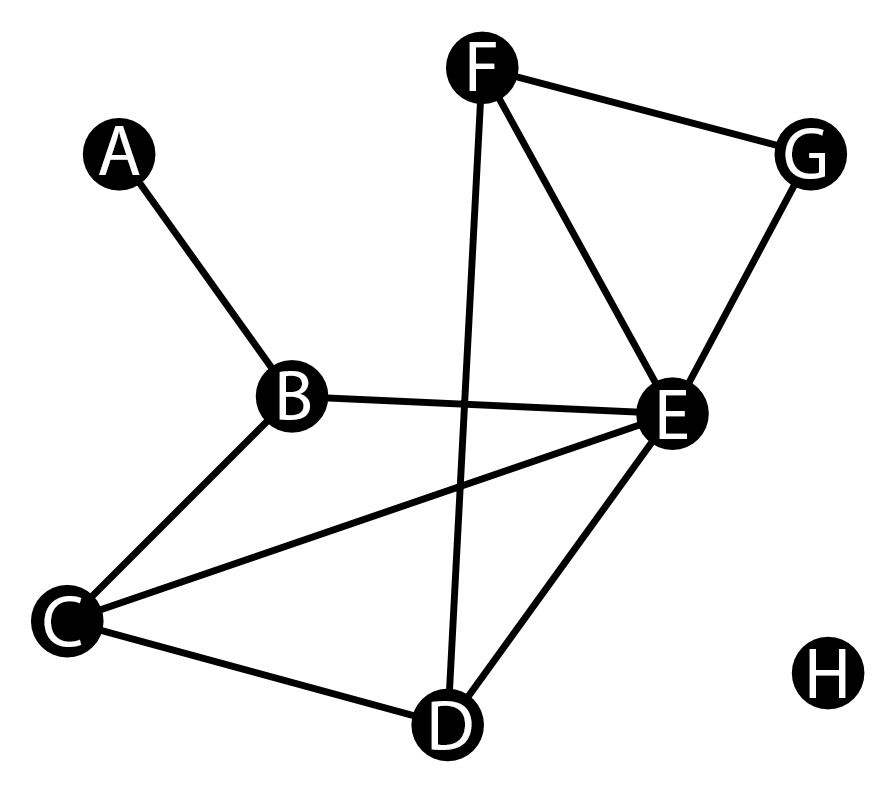
\includegraphics[width=0.25\textwidth]{week_02_lecture_img_01}
  \end{center}    
  \begin{itemize}
    \item The degree of a vertex is the number of edges attached to it. 
    \item In a directed network, we can distinguish between in-degree and out-degree.
    \item The degree can range from 0 (isolated vertex) up to $n-1$, where $n$ is the total number of vertices.
  \end{itemize}

\end{frame}


\begin{frame}{Degree distribution}
  \begin{center}
    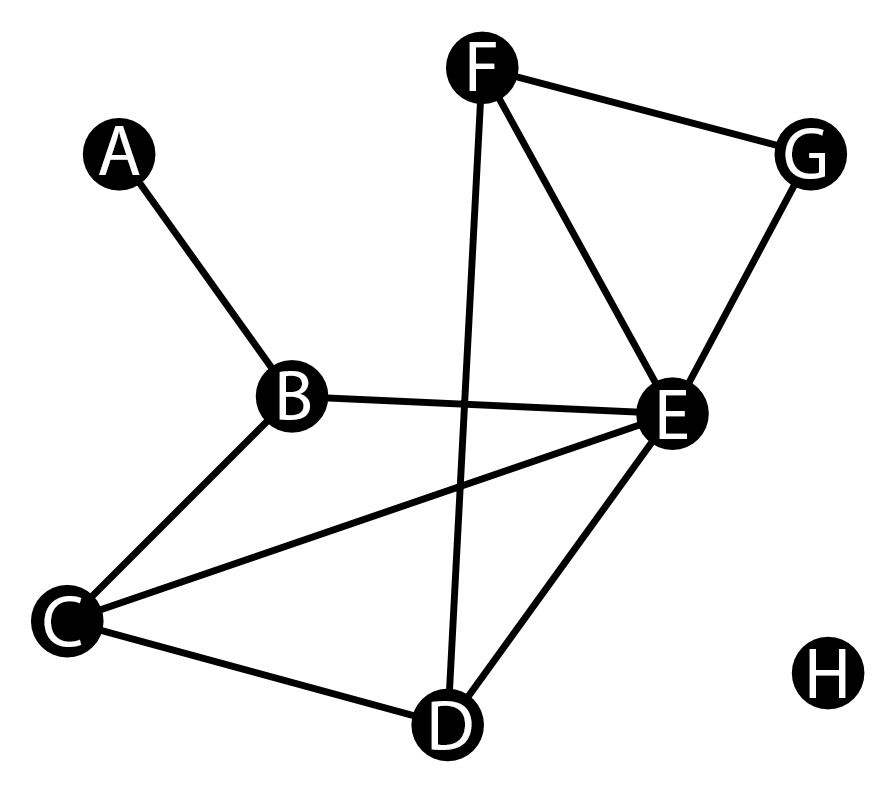
\includegraphics[width=0.25\textwidth]{week_02_lecture_img_01}
  \end{center}    
  \begin{itemize}
    \item Let's list all the degrees of the network above: $0, 1, 2, 2, 3, 3, 3, 4$.
    \item The (empirical) degree distribution is the frequency (count) of each degree in the network.
    \begin{table}
      \centering
      \begin{tabular}{lccccccc}
        \toprule
        Degree    & 0 & 1 & 2 & 3 & 4 & 5 & $\cdots$\\
        \midrule
        Frequency & 1 & 1 & 1 & 4 & 0 & 1 & $\cdots$\\
        \bottomrule
      \end{tabular}
    \end{table}
    \item The degree is a measure of the importance of a vertex in a network. The higher the degree, the more important the vertex. 
    \item An example of this is the number of subscribers/followers/connections on a social media platform.
    \item The degree distribution is considered one of the most important properties of a network, although it actually tells us very little about the structure of the network.
  \end{itemize}

\end{frame}



\begin{frame}{Edge Density}
  \begin{center}
    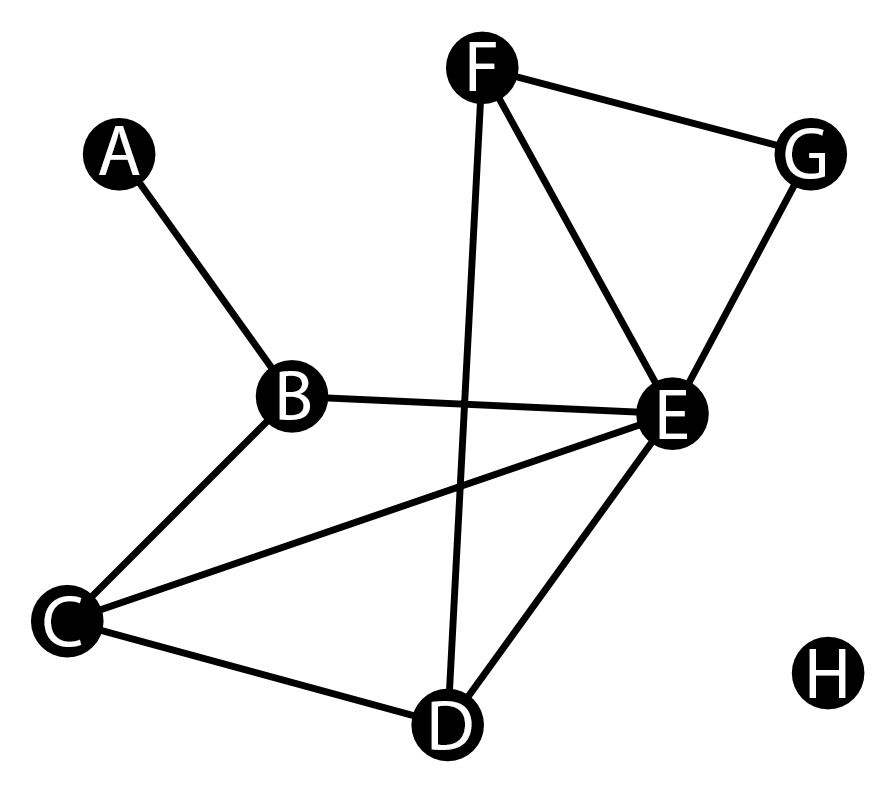
\includegraphics[width=0.25\textwidth]{week_02_lecture_img_01}
  \end{center}    
  \begin{itemize}
    \item Edge density is a measure of how connected a network is \emph{on average}.
    \item It is defined as the ratio of the number of edges to the maximum possible number of edges in the network.
    \item For an undirected simple graph with $n$ vertices, the maximum number of edges is ${n\choose 2} = \frac{n(n-1)}{2}$.
    \item Edge density ranges from 0 (no edges) to 1 (fully connected network).
    \item In the network above, the edge density is $\frac{9}{{8\choose 2}} \approx 0.32$.
  \end{itemize}
\end{frame}



\begin{frame}{Sparse and Dense Graphs}
  \begin{itemize}
    \item The edge density can serve as a (crude) way to classify (large) graphs.
    \item Sparse graphs have low edge density, dense graphs have high edge density.
    \item Different research communities have different definitions of what constitutes a sparse or dense graph.
    \item Dense typically means that the number of edges is of order $n^2$, which means the average degrees are of order $n$.
    \item Sparse typically means that the number of edges is of order $n$, which means the average degrees are of order 1.
    \item The disargeement is mostly about what we call those graphs in between.
    \item The distinction between dense and sparse is important to develop mathematical theories of graphs, but for any finite graph, it is hard to argue whether it is dense or sparse.
  \end{itemize}
\end{frame}

\begin{frame}{Measuring the importance of vertices}
  \begin{itemize}
    \item \emph{Centrality measures} quantify the importance or influence of a vertex in a network. 
    \item These vertices play crucial roles in the network structure.
    \item There are different centrality measures, each capturing a different aspect of importance.
  \end{itemize}
\end{frame}

\begin{frame}{Betweenness Centrality}
  \begin{itemize}
    \item Betweenness centrality is a measure of the extent to which a vertex lies on the shortest paths between other vertices in a network.
    \item Vertices with high betweenness centrality are often considered as ``brokers'' or ``gatekeepers'' in the network, as they have the potential to control the flow of information between different parts of the network.
    \item The betweenness centrality of a vertex $v$ is calculated as the sum of the fractions of shortest paths between all pairs of vertices that pass through $v$:
    \[
    C_B(v) = \sum_{s \neq v \neq t} \frac{\sigma_{st}(v)}{\sigma_{st}}
    \]
    where $\sigma_{st}$ is the total number of shortest paths between vertices $s$ and $t$, and $\sigma_{st}(v)$ is the number of those paths that pass through $v$.
    \item Betweenness centrality is only defined for vertices with degree at least 2.
  \end{itemize}
\end{frame}


\begin{frame}{Betweenness Centrality}
  \begin{center}
    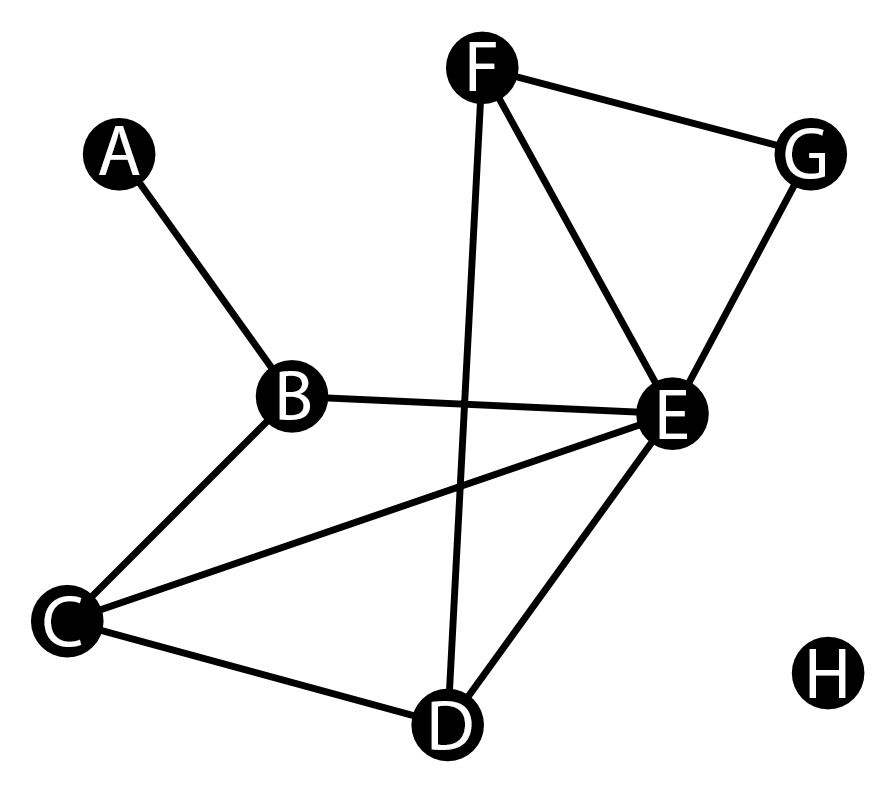
\includegraphics[width=0.25\textwidth]{week_02_lecture_img_01}
  \end{center}    
  \begin{itemize}
    \item Let's calculate the betweenness centrality of vertex E in the network above. In the following table, the first number is the number of shortest paths that pass through E, the second number is the total number of shortest paths between the two vertices.
    \item A--B: 0,1; A--C: 0,1; A--D; 1,2; A--F: 1,1; A--G; 1,1; B--C: 0,1; B--D: 1,2; B--F: 1,1; B--G: 1,1; C--D: 0,1; C--F: 1,1; C--G: 1,1; D--F: 0,1; D--G: 1,2; F--G: 0,1. 
    \item Hence, the betweenness centrality of E is $9/18$.  
  \end{itemize}
\end{frame}

\begin{frame}{Betweenness Centrality}
  \begin{center}
    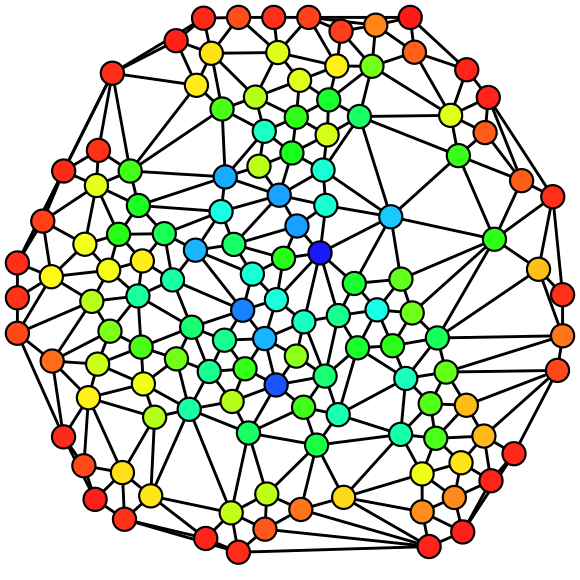
\includegraphics[width=0.4\textwidth]{week_02_lecture_img_02}
  \end{center}    
  \begin{itemize}
    \item In this graph, red vertices have the lowest betweenness centrality, while blue vertices have the highest betweenness centrality.
  \end{itemize}
\end{frame}

\begin{frame}{Closeness Centrality}
  \begin{itemize}
    \item Closeness centrality is a measure of how close a vertex is to all other vertices in a network.
    \item Vertices with high closeness centrality are able to quickly access information from other parts of the network.
    \item The closeness centrality of a vertex $v$ is calculated as the reciprocal of the average shortest path length from $v$ to all other vertices:
    \[
    C_C(v) = \frac{1}{\sum_{u \neq v} d(v,u)}
    \]
    where $d(v,u)$ is the shortest path length between vertices $v$ and $u$.
    \item Closeness centrality is defined for all vertices in a connected network.
  \end{itemize}
\end{frame}

\begin{frame}{Closeness Centrality}
  \begin{center}
    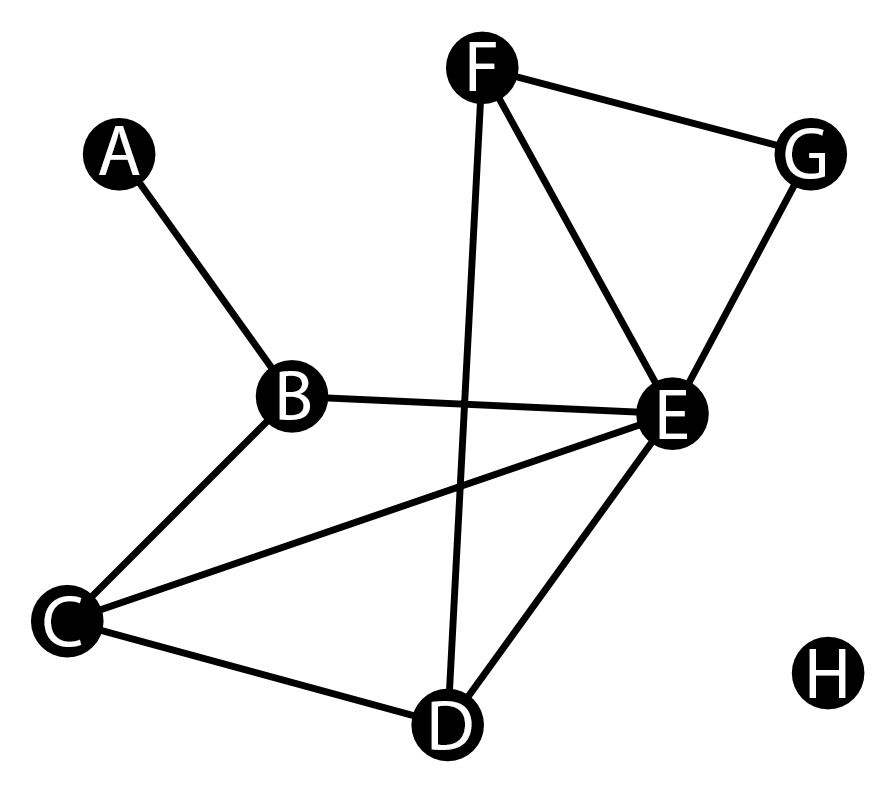
\includegraphics[width=0.25\textwidth]{week_02_lecture_img_01}
  \end{center}    
  \begin{itemize}
    \item Let's calculate the closeness centrality of vertex E in the network above within its connected component.
    \item The shortest path lengths from E to all other vertices are: A--E: 2, B--E: 1, C--E: 1, D--E: 1, F--E: 1, G--E: 1.
    \item Hence, the closeness centrality of E is $6/(2+1+1+1+1+1)=6/7$.  
    \item The closeness centrality of A is $6/(1+2+3+2+3+3)=6/14$. 
  \end{itemize}
\end{frame}


\begin{frame}{Eigenvector Centrality}
  \begin{itemize}
    \item Eigenvector centrality is a measure of the importance of a vertex in a network based on the concept of eigenvectors.
    \item It takes into account not only the number of connections a vertex has, but also the importance of those connections.
    \item The eigenvector centrality of a vertex $v$ is calculated as the principal eigenvector of the adjacency matrix of the network:
    \[
    \mathbf{Ax} = \lambda \mathbf{x}
    \]
    where $\mathbf{A}$ is the adjacency matrix, $\mathbf{x}$ is the eigenvector, and $\lambda$ is the largest eigenvalue of $A$.
    \item The eigenvector is unique up to a scaling factor if the network is connected and it can be shown that all its entries are positive.
  \end{itemize}
\end{frame}

\begin{frame}{Eigenvector Centrality}
  \begin{center}
    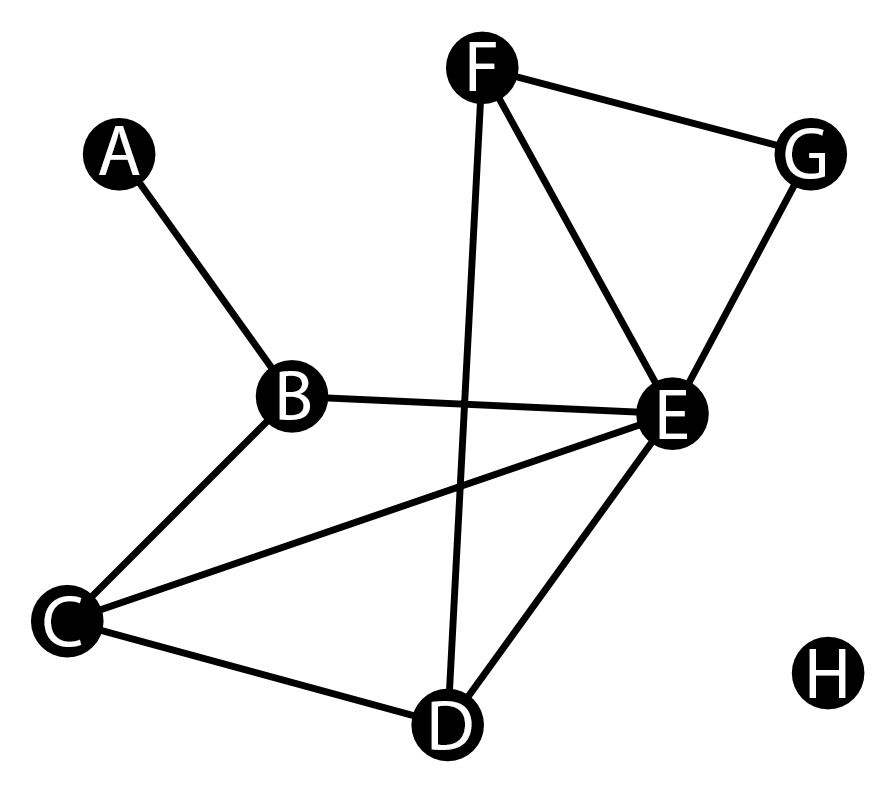
\includegraphics[width=0.25\textwidth]{week_02_lecture_img_01}
  \end{center}    
  \begin{itemize}
    \item Let's calculate the eigenvector centrality of vertex E in the network above.
    \item The adjacency matrix $\mathbf{A}$ of the connected component containing E is:
    \[
    \mathbf{A} = \scriptsize\begin{bmatrix}
    0 & 1 & 0 & 0 & 0 & 0 & 0 \\
    1 & 0 & 1 & 0 & 1 & 0 & 0 \\
    0 & 1 & 0 & 1 & 1 & 0 & 0 \\
    0 & 0 & 1 & 0 & 1 & 1 & 0 \\
    0 & 1 & 1 & 1 & 0 & 1 & 1 \\
    0 & 0 & 0 & 1 & 1 & 0 & 1 \\
    0 & 0 & 0 & 0 & 1 & 1 & 0 \\
    \end{bmatrix}
    \]
    \item Solving the equation $\mathbf{Ax} = \lambda \mathbf{x}$, we obtain for the largest eigenvalue that   
    \[
    \lambda \approx 3.253,\qquad \mathbf{x} \approx \scriptsize\begin{bmatrix}
      0.100 \\
      0.326 \\
      0.400 \\
      0.415 \\
      0.560 \\
      0.390 \\
      0.292 \\
      \end{bmatrix}
    \]
  \end{itemize}
\end{frame}

\begin{frame}{PageRank}
  \begin{itemize}
    \item PageRank is an algorithm used by Google to rank web pages in their search engine results.
    \item It is based on the idea of random walks on a directed network produced by links from one webpage to another.
    \item A random walker starts at any vertex, and at each step, moves to a neighboring vertex with equal probability.
    \item The probability of being at a particular vertex after a large number of steps is the PageRank of that vertex.
    \item The long-term probabilities are closely related to the eigenvector centrality, but we won't go into the details here. 
    \item PageRank also uses a damping factor to avoid the problem of ``spider traps'' and ``dead ends''. At any step, the walker may with a small probability (about 0.15) decide to jump to a randomly chosen vertex.
  \end{itemize}
\end{frame}


\begin{frame}{Triangles and Cluster Coefficient}
  \begin{center}
    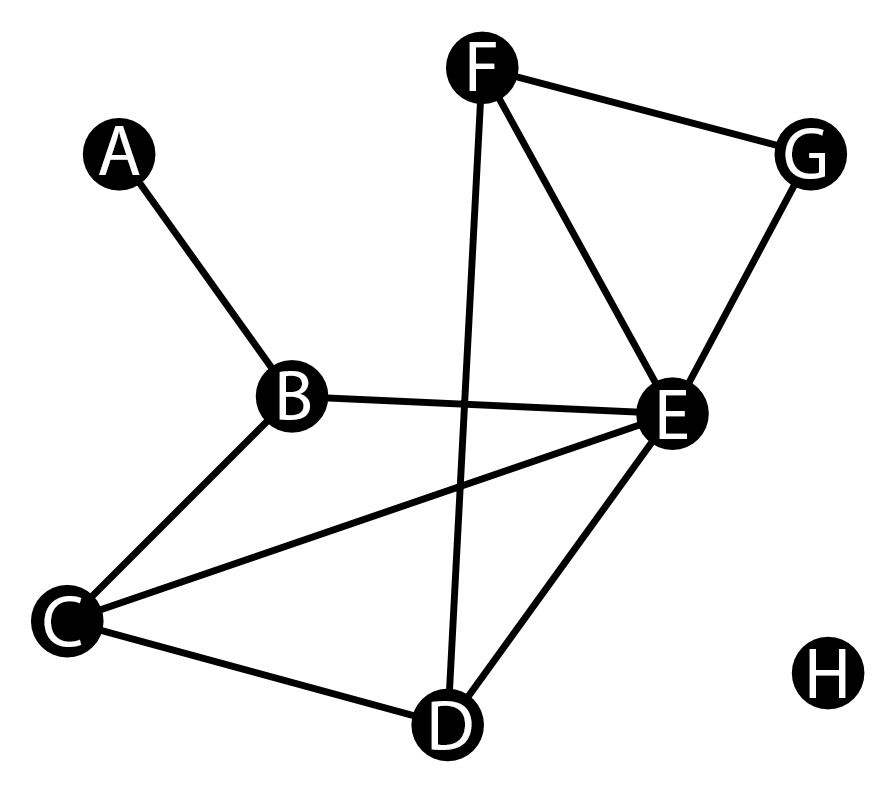
\includegraphics[width=0.25\textwidth]{week_02_lecture_img_01}
  \end{center}    
  \begin{itemize}
    \item A triangle consists of three vertices connected by three edges, also called 3-cycle.
    \item Clustering refers to the tendency of vertices to form tightly interconnected groups or communities.
    \item The presence of triangles in a network indicates a higher level of clustering (``my friends are more likely to be friends with each other'').
    \item The cluster coefficient can be calculated as
    \[
    C = \frac{{3 \times \text{{number of triangles}}}}{{\text{{number of 2-paths}}}}
    \]
    \item A 2-star are three vertices connected by (at least) two edges. The number of 2-stars equals $\sum_v {d_v \choose 2}$, where $d_v$ is the degree of vertex $v$.  
    \item In the network above, the cluster coefficient is $3\times4/18$.
  \end{itemize}
\end{frame}


\begin{frame}{Similarity}
  \begin{center}
    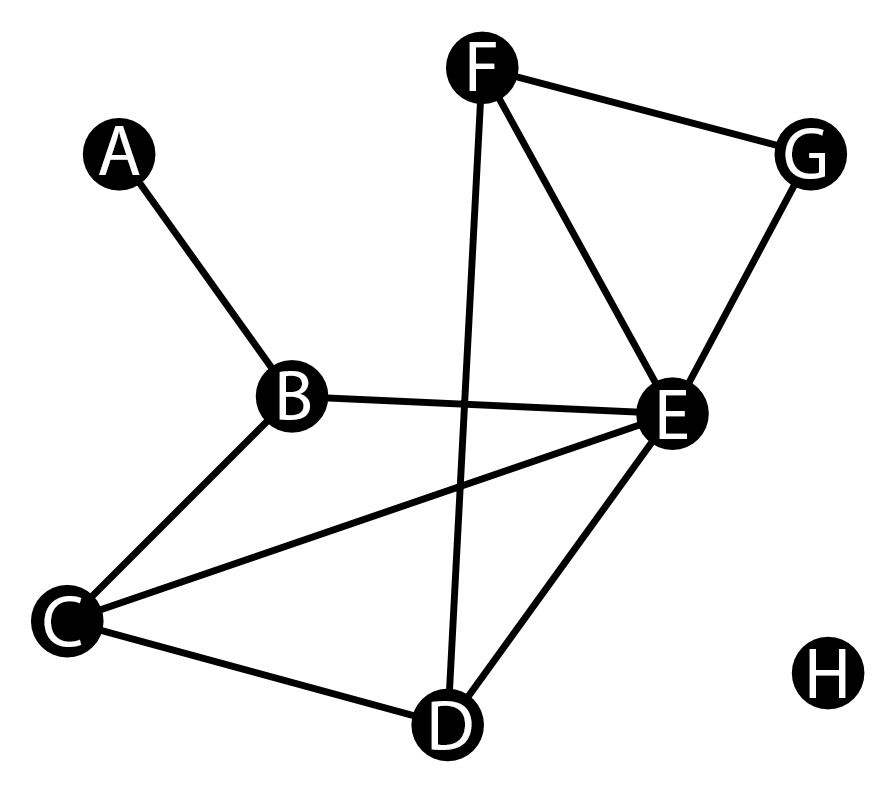
\includegraphics[width=0.25\textwidth]{week_02_lecture_img_01}
  \end{center}    
  \begin{itemize}
    \item Similarity can be defined based on various aspects of the network structure.
    \item One common measure of similarity is \emph{neighborhood overlap}.
    \item Neighborhood overlap between two vertices is the fraction of common neighbors they share and provides a measure of how similar their local network structures are.
    \item In the graph above, the neighborhood overlap between vertices B and E is 1/7, so they have low similarity.
    \item There are many other ways to define similarity.
  \end{itemize}
\end{frame}


\begin{frame}{Assortativity and Mixing}
  \begin{center}
    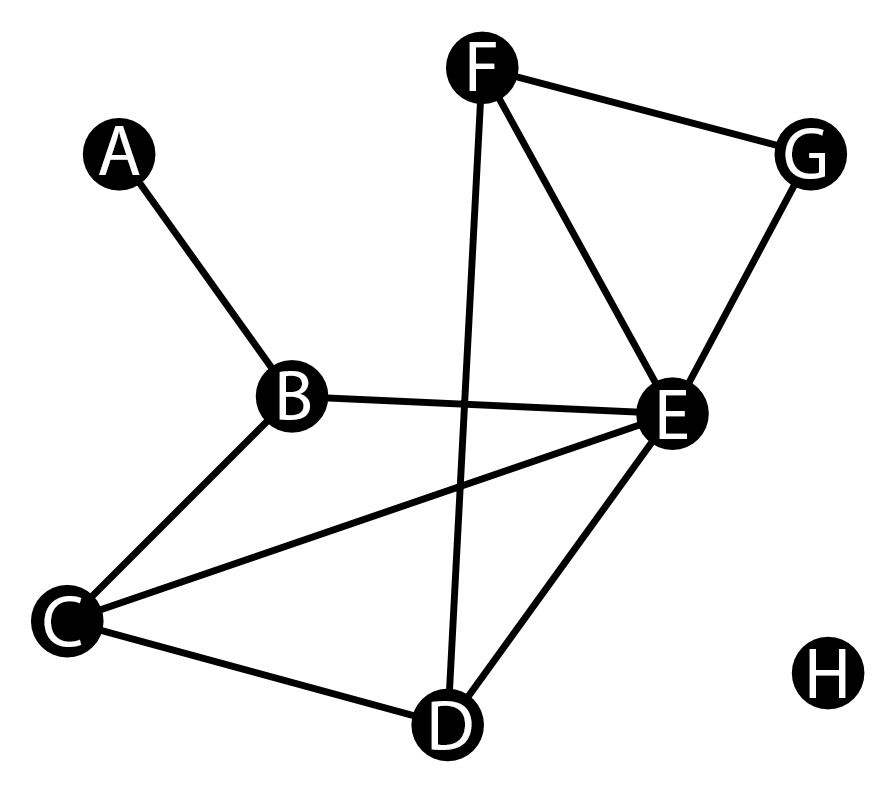
\includegraphics[width=0.25\textwidth]{week_02_lecture_img_01}
  \end{center}    
  \begin{itemize}
    \item Assortativity and mixing are measures that describe the patterns of connections between different types of vertices in a network.
    \item Assortativity refers to the tendency of vertices to connect to similar vertices, while disassortativity refers to the tendency of vertices to connect to dissimilar vertices.
    \item Assortativity can be measured using various metrics, such as the degree assortativity coefficient or the attribute assortativity coefficient.
    \item The degree assortativity coefficient is the correlation between the degrees of connected vertices. 
    \item In the grah above, degree correlation is about -0.25, so the network is degree disassortative.
  \end{itemize}
\end{frame}




\end{document}

